% XCircuit output "vas.tex" for LaTeX input from vas.eps
\def\putbox#1#2#3#4{\makebox[0in][l]{\makebox[#1][l]{}\raisebox{\baselineskip}[0in][0in]{\raisebox{#2}[0in][0in]{\scalebox{#3}{#4}}}}}
\def\rightbox#1{\makebox[0in][r]{#1}}
\def\centbox#1{\makebox[0in]{#1}}
\def\topbox#1{\raisebox{-0.60\baselineskip}[0in][0in]{#1}}
\def\midbox#1{\raisebox{-0.20\baselineskip}[0in][0in]{#1}}
   \scalebox{1}{
   \normalsize
   \parbox{5.92708in}{
   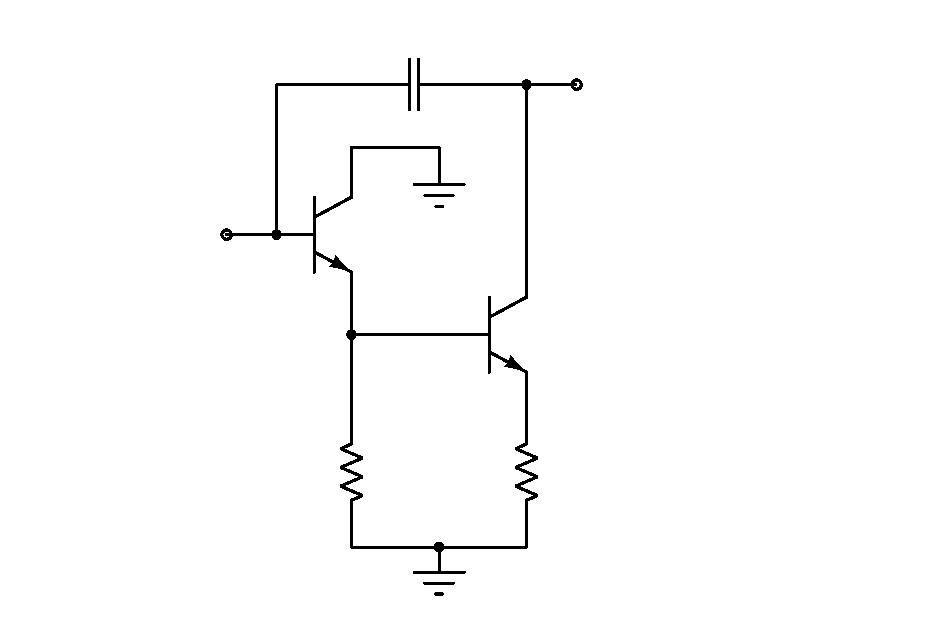
\includegraphics[scale=1]{vas}\\
   % translate x=770 y=524 scale 0.38
   \putbox{2.23in}{2.45in}{1.20}{\midbox{$Q_{43}$}}%
   \putbox{3.48in}{1.79in}{1.20}{\midbox{$Q_{20}$}}%
   \putbox{3.57in}{0.87in}{1.20}{\midbox{$R_{23}$}}%
   \putbox{2.40in}{0.87in}{1.20}{\midbox{$R_{46}$}}%
   \putbox{2.65in}{3.70in}{1.20}{\centbox{$C_{10}$}}%
   \putbox{1.32in}{2.45in}{1.20}{\rightbox{\midbox{$v_{O_{pd}}$}}}%
   \putbox{3.90in}{3.45in}{1.20}{\midbox{$v_{O_{\textit{vas}}}$}}%
   } % close 'parbox'
   } % close 'scalebox'
   \vspace{-\baselineskip} % this is not necessary, but looks better
